\begin{appendices}
    \chapter{Additional Results} \label{app:additionalResults}
    \section{Validation Results} \label{app:verifResults}

    \begin{figure}[H]
    \centering
    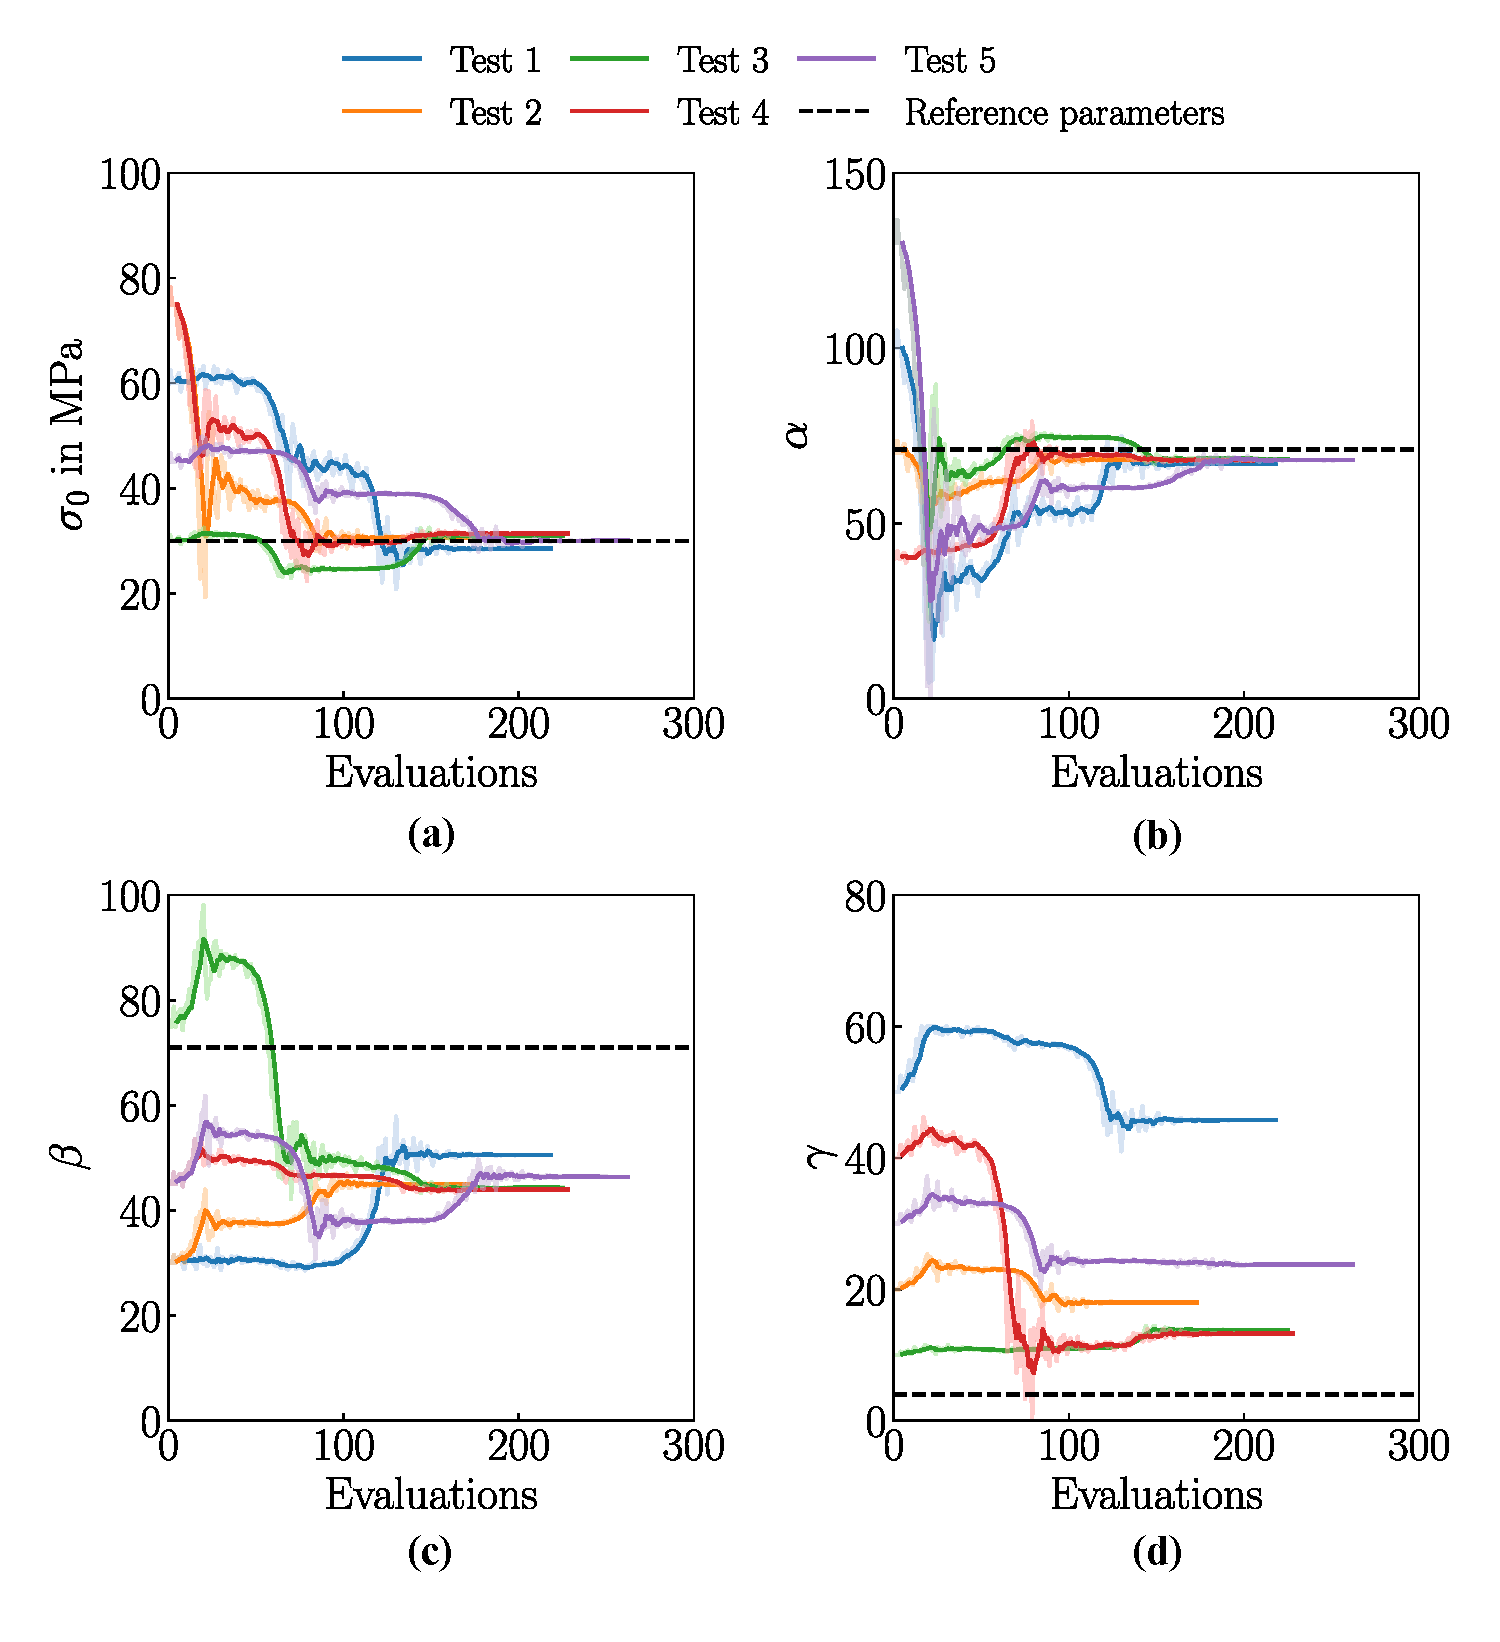
\includegraphics[width=0.66\textwidth]{Vald_4To3_fixEP1_material_params.pdf}
    \caption{Evolution of the optimised material parameters: (a) yield stress $\sigma_0$; hardening coefficients (b) $\alpha$; (c) $\beta$; (d) $\gamma$; over the optimisation evaluations for material with mixing ratio 4:3 under linear tensile strain with respective reference values obtained by \citet{ries_deciphering_nodate} and predefined elastic parameters Young's modulus $E$ and Poisson's ratio $\nu$}
    \label{fig:material_params_4to3}
    \end{figure}

    \begin{figure}[H]
    \centering
    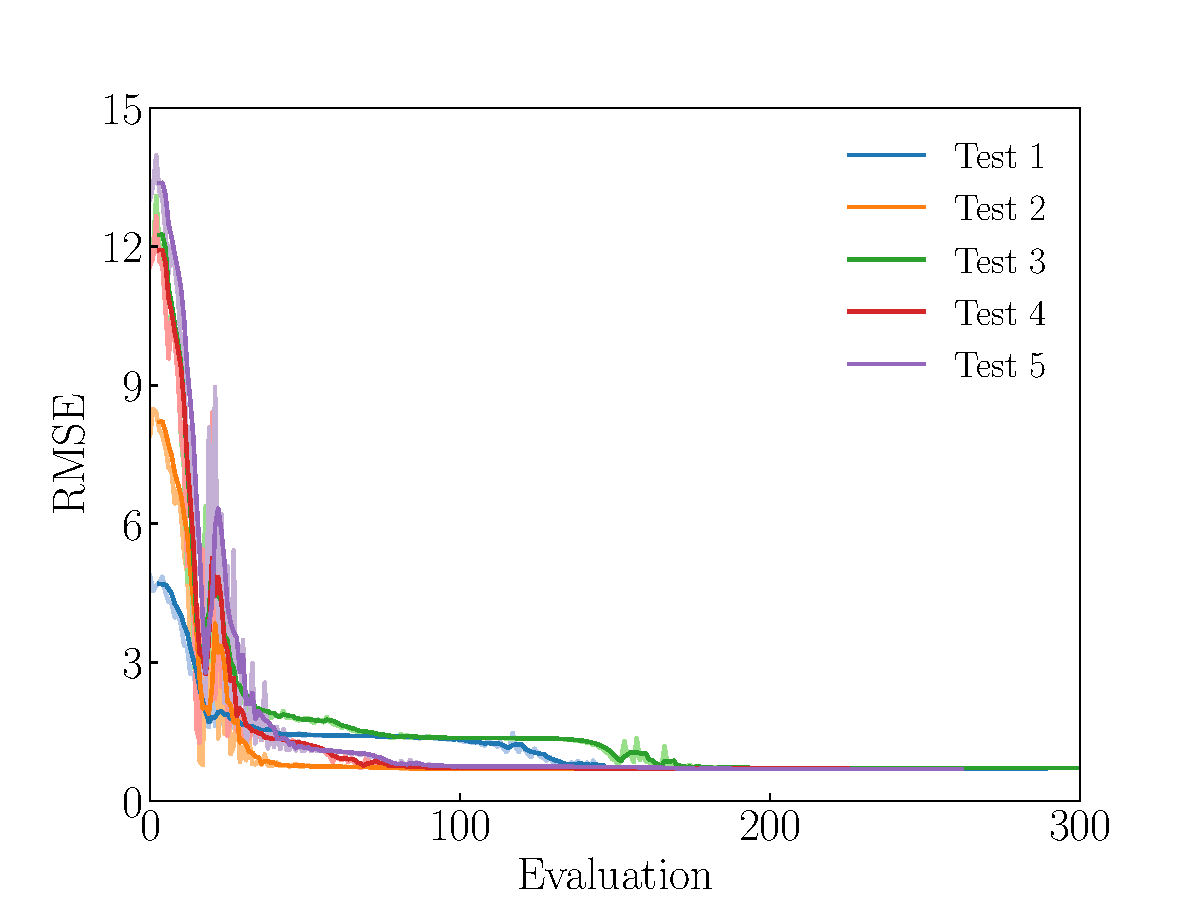
\includegraphics[width=0.5\textwidth]{Vald_4To3_fixEP1_rsme_lin_plot.pdf}
    \caption{Evolution of the \acrfull{rmse} during the optimisation for all tests for material with mixing ratio 4:3 under linear tensile strain}
    \label{fig:verfifRMSE43}
    \end{figure}

    \begin{figure}[H]
    \centering
    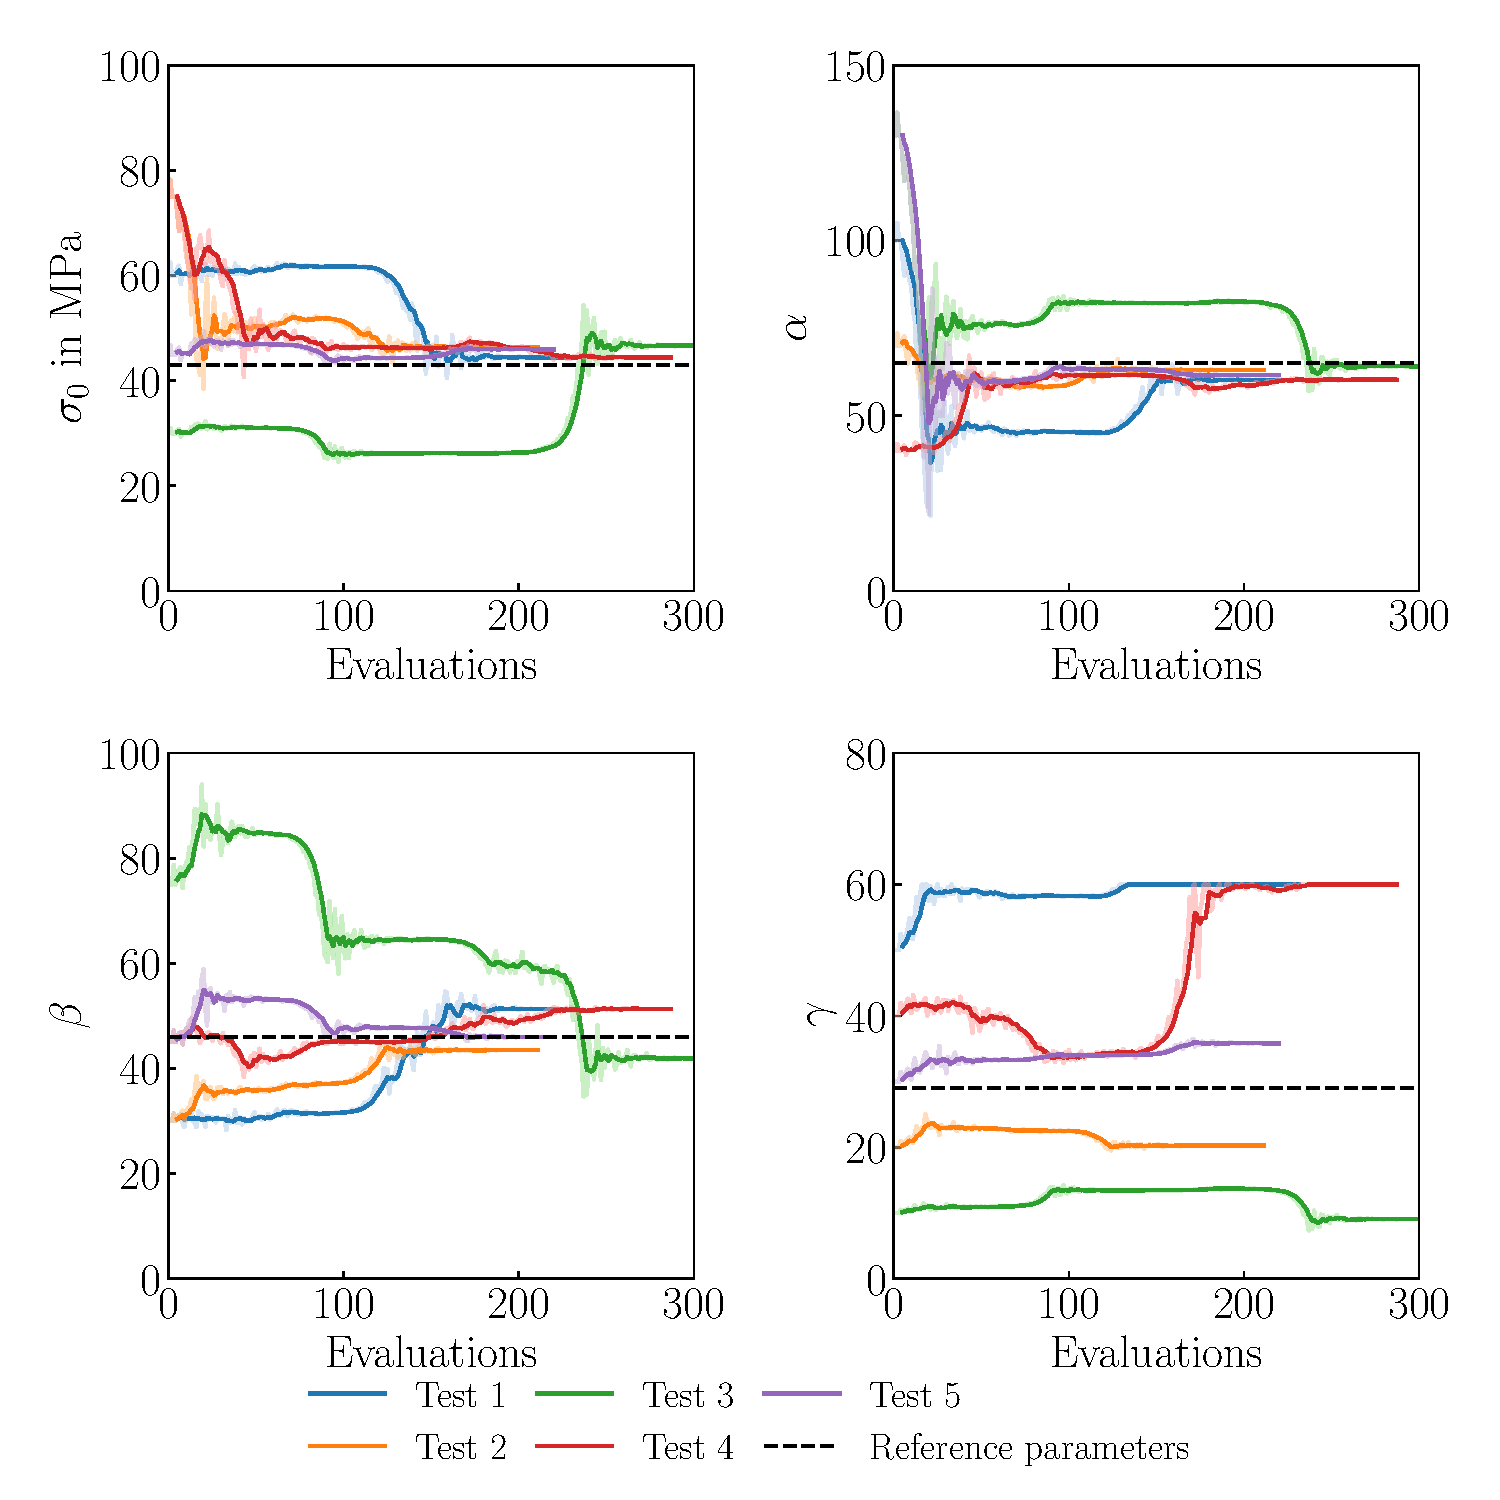
\includegraphics[width=0.66\textwidth]{Vald_8To3_fixEP1_material_params.pdf}
    \caption{Evolution of the optimised material parameters: (a) yield stress $\sigma_0$; hardening coefficients (b) $\alpha$; (c) $\beta$; (d) $\gamma$; over the optimisation evaluations for material with mixing ratio 8:3 under linear tensile strain with respective reference values obtained by \citet{ries_deciphering_nodate} and predefined elastic parameters Young's modulus $E$ and Poisson's ratio $\nu$}
    \label{fig:material_params_8to3}
    \end{figure}

    \begin{figure}[H]
    \centering
    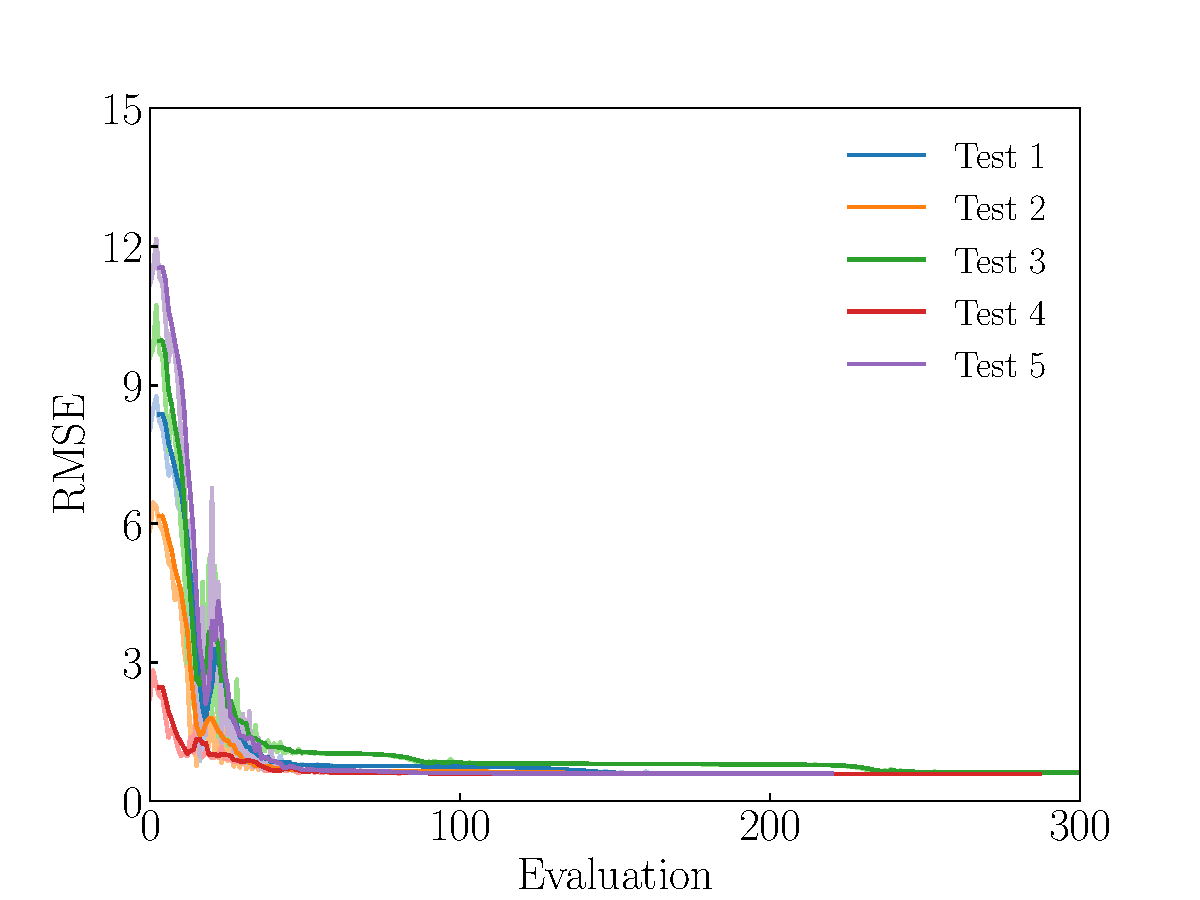
\includegraphics[width=0.5\textwidth]{Vald_8To3_fixEP1_rsme_lin_plot.pdf}
    \caption{Evolution of the \acrfull{rmse} during the optimisation for all tests for material with mixing ratio 8:3 under linear tensile strain}
    \label{fig:verfifRMSE83}
    \end{figure}


    \section{Tensile-Shear combination Results} \label{app:tensileShearResults}
    \begin{figure}[H]
    \centering
    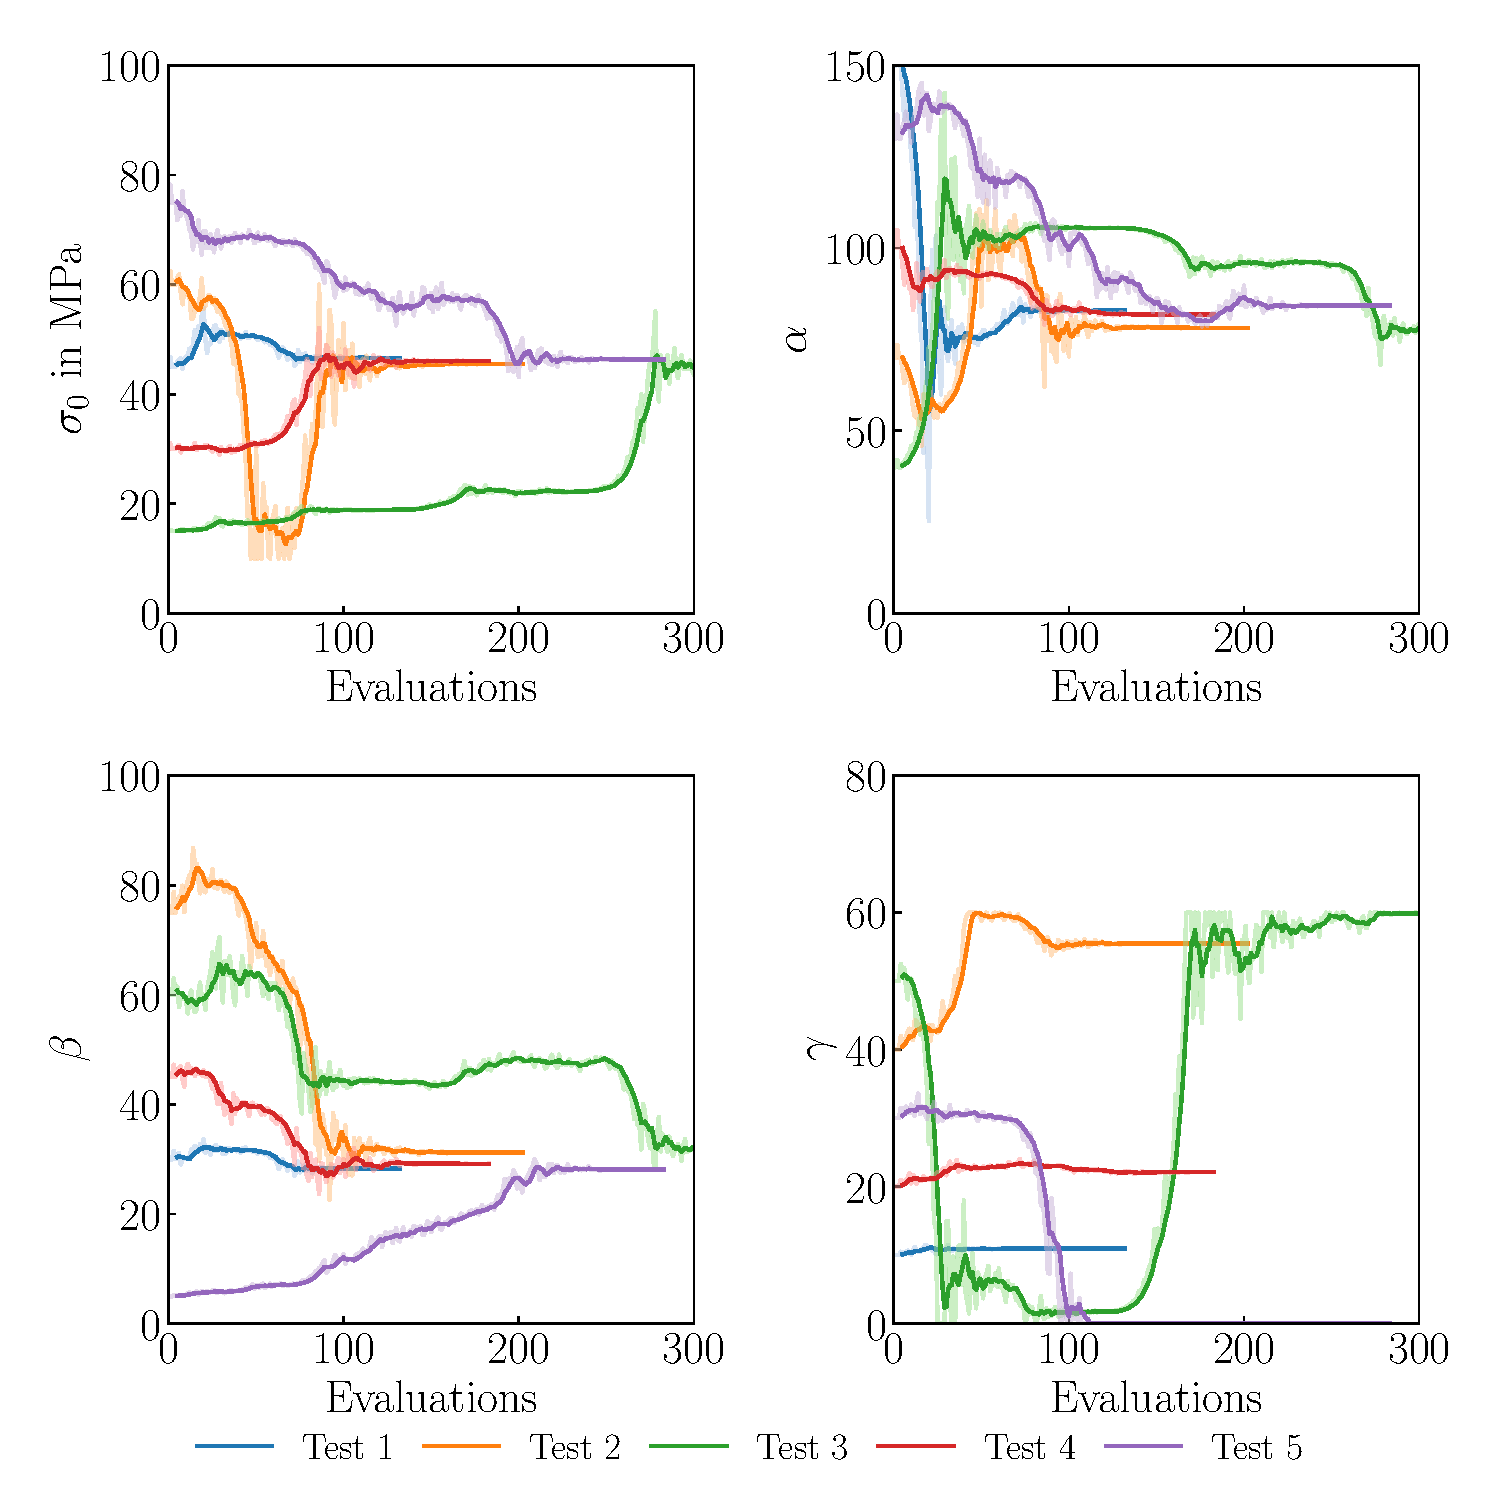
\includegraphics[width=0.7\textwidth]{Tensile_6to3_015_fixENu_material_params.pdf}
    \caption{Evolution of the optimised material parameters: (a) yield stress $\sigma_0$; hardening coefficients (b) $\alpha$; (c) $\beta$; (d) $\gamma$; over the optimisation evaluations for material with mixing ratio 6:3 under pure sinusoidal tensile strain and predefined elastic parameters Young's modulus $E$ and Poisson's ratio $\nu$}
    \label{fig:tensileMatParams}
    \end{figure}

    \begin{figure}[H]
    \centering
    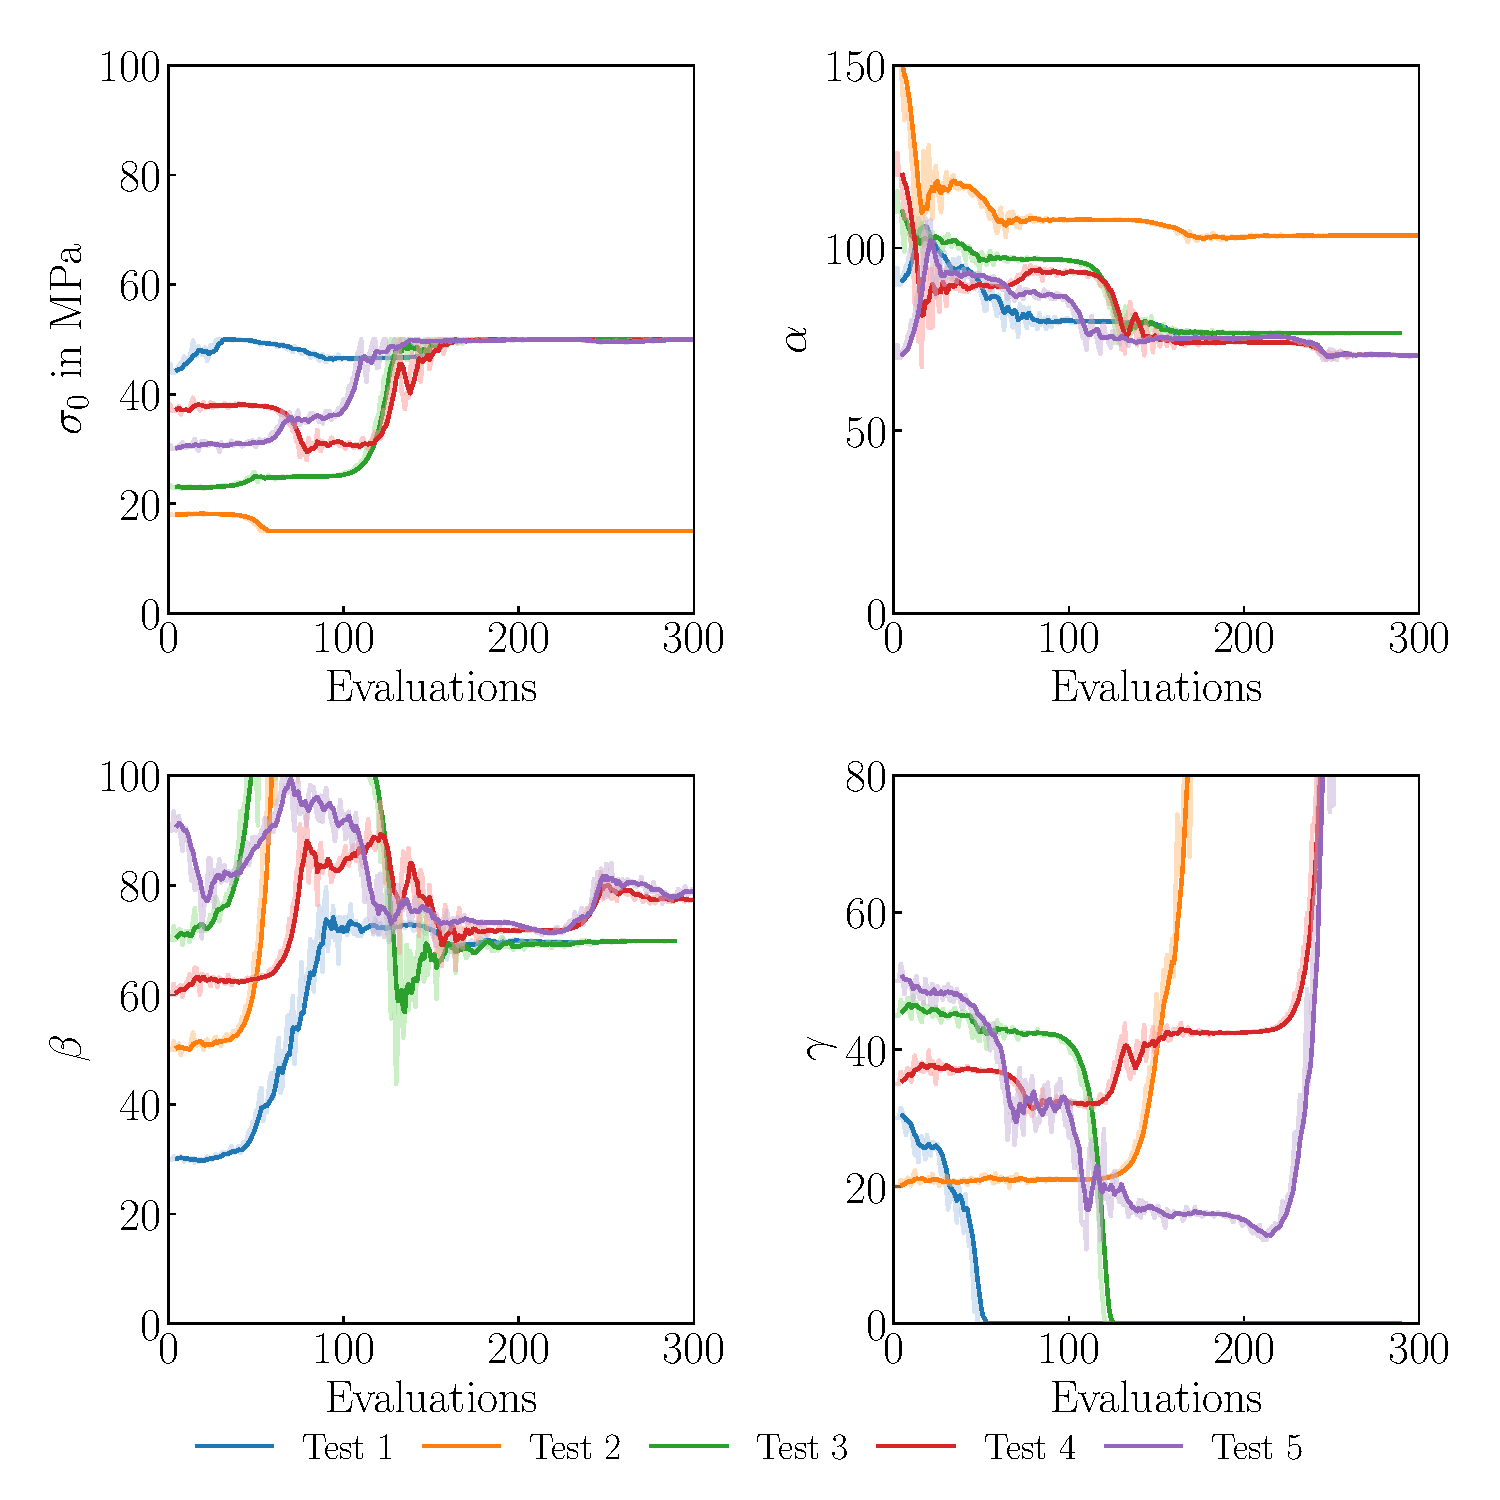
\includegraphics[width=0.7\textwidth]{Shear_6to3_015_fixENu_500_material_params.pdf}
    \caption{Evolution of the optimised material parameters: (a) yield stress $\sigma_0$; hardening coefficients (b) $\alpha$; (c) $\beta$; (d) $\gamma$; over the optimisation evaluations for material with mixing ratio 6:3 under pure sinusoidal shear strain and predefined elastic parameters Young's modulus $E$ and Poisson's ratio $\nu$}
    \label{fig:shearMatParams}
    \end{figure}


    XX STRAIN STRAIN FÜR VALIDIERUNGSVERSUCHE
    XX CODE UND INPUT FILE
    \chapter{Appendix}
\end{appendices}